\documentclass[]{article}
\renewcommand{\baselinestretch}{1.25}

\usepackage[margin=1in]{geometry}
\usepackage{physics}
\usepackage{amsmath, amsfonts, amssymb, amsthm}
\usepackage{amssymb}
\usepackage{graphicx}
\usepackage{hyperref}
\usepackage{empheq}


% MATLAB Formatting Code
\usepackage[numbered,framed]{matlab-prettifier}
\lstset{style=Matlab-editor,columns=fullflexible}
\renewcommand{\lstlistingname}{Script}
\newcommand{\scriptname}{\lstlistingname}

% TikZ Things
\usepackage{tikz}
\usetikzlibrary{positioning,shapes}


% Formatting Preferences
\numberwithin{equation}{section}
\usepackage{parskip}
\renewcommand{\figurename}{Fig.}
\allowdisplaybreaks

% Section Heading Settings
\usepackage{enumitem}
\renewcommand{\theenumi}{\alph{enumi}}
\renewcommand*{\thesection}{Problem \arabic{section}}
\renewcommand*{\thesubsection}{\alph{subsection})}
\renewcommand*{\thesubsubsection}{\quad \quad \roman{subsubsection})}

% Math Proof things
\newcommand{\Rel}{\mathcal{R}}
\newcommand{\R}{\mathbb{R}}
\newcommand{\C}{\mathbb{C}}
\newcommand{\N}{\mathbb{N}}
\newcommand{\Z}{\mathbb{Z}}
\newcommand{\Q}{\mathbb{Q}}

\newcommand{\st}{\ : \ }

% Theorem Definition
\newtheorem{definition}{Definition}
\newtheorem{assumption}{Assumption}
\newtheorem{theorem}{Theorem}
\newtheorem{lemma}{Lemma}
\newtheorem{proposition}{Proposition}
\newtheorem{example}{Example}


% Multiagent Robotic Systems Commands
\newcommand{\diam}{\text{diam}}
\newcommand{\radius}{\text{radius}}




%opening
\title{MECH 6V29: Multiagent Robotic Systems- HW 1}
\author{Jonas Wagner}
\date{2022, Febuary 10\textsuperscript{th}}

\begin{document}	

\maketitle

% \tableofcontents

%----------------------------------------------------------------------------

% Problem 1 -------------------------------------------------
% \newpage
\section{}
% \textbf{Problem:} 
State a summary of first five lectures, preferably by creating a concept map diagram (flow diagram). 
The whole purpose is to make sure that we are clear about the bigger picture, 
and reiterate why are we doing and discussing the specific topics in the class. 
Do not merely write the topics, instead create connections between topics to clarify the flow of information.

\subsection*{Big Picture Chart}
\begin{figure}[h]
	\centering
	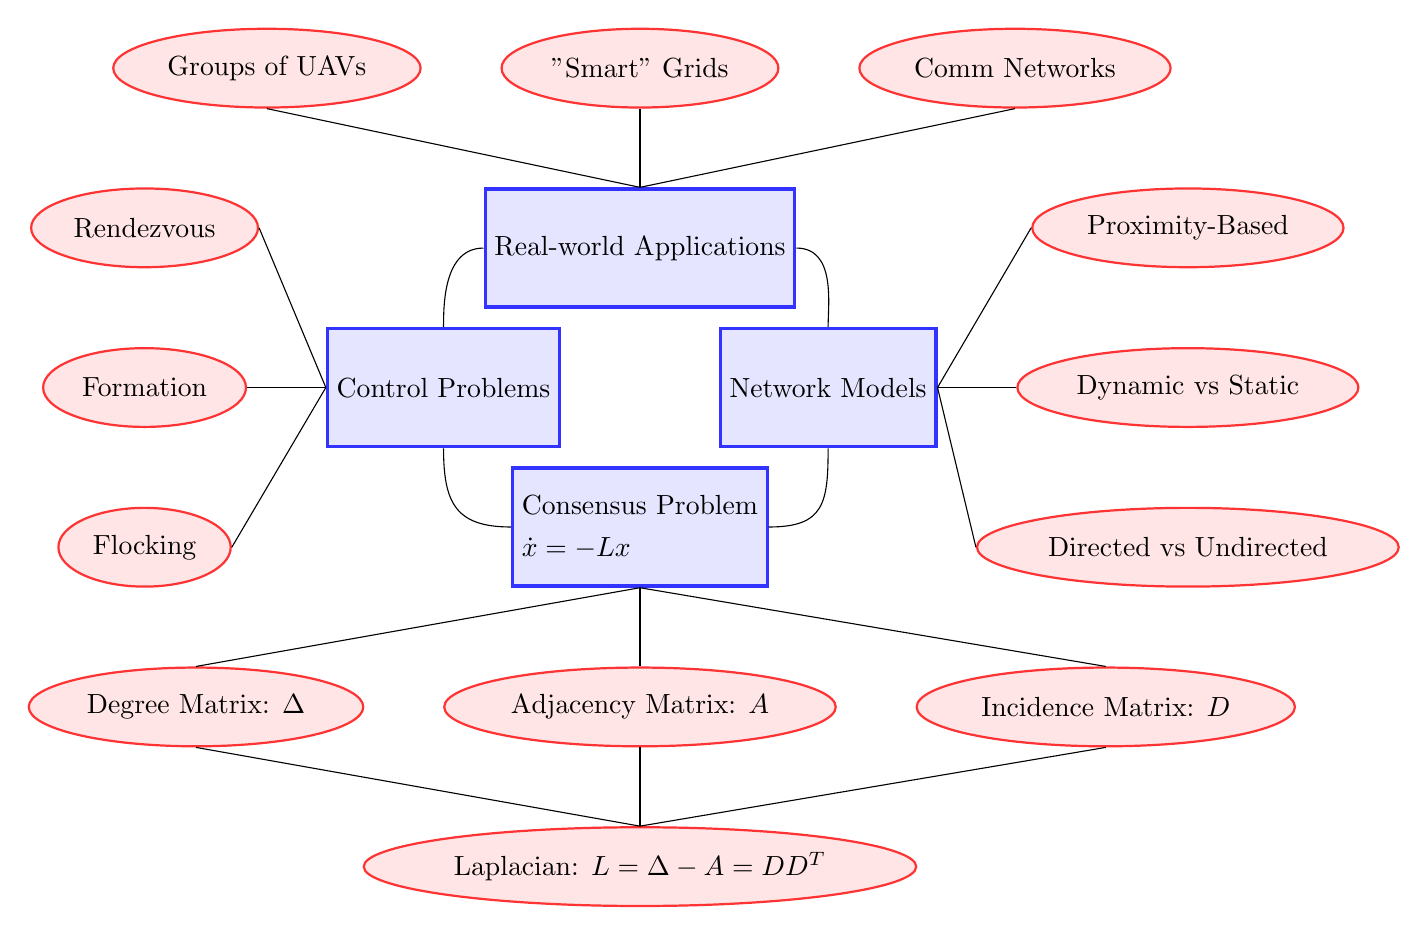
\begin{tikzpicture}[
		empty/.style={coordinate, draw=white!0, fill=white!0, thin, minimum size = 0.1mm},
		block/.style={rectangle, draw=blue!80, fill=blue!10, very thick, minimum size = 15mm},
		extra/.style={ellipse, draw=red!80, fill=red!10, thick, minimum size = 10mm},
		auto,
		% roundnode/.style={circle, draw=green!60, fill=green!5, very thick, minimum size=7mm},
		% squarednode/.style={rectangle, draw=red!60, fill=red!5, very thick, minimum size=5mm},
		]
		%Main Nodes
		\node[empty]	(center)								{};
		\node[block]	(applications)		[above=of center]	{Real-world Applications};
		\node[block]	(ctrl_pblms)		[left=of center] 	{Control Problems};
		\node[block]	(network_model)		[right=of center] 	{Network Models};
		\node[block, text width = 30mm]	(consensus)			[below=of center]	{Consensus Problem $\dot{x}=-L x$};

		%Main Lines
		\draw[-] (applications.west) 	.. controls +(left:5mm) and +(up:3mm)  ..	(ctrl_pblms.north); %controls +(up:5mm) and +(left:5mm)
		\draw[-] (applications.east) 	.. controls +(right:5mm) and +(up:3mm) .. (network_model.north);
		\draw[-] (ctrl_pblms.south) 	.. controls +(down:7mm) and +(left:7mm)  .. (consensus.west);
		\draw[-] (network_model.south)	.. controls +(down:7mm) and +(right:7mm) ..	(consensus.east);

		%Applications
		\node[extra]	(app_2)		[above=of applications]	{"Smart" Grids};
		\node[extra]	(app_1)		[left=of app_2]			{Groups of UAVs};
		\node[extra]	(app_3)		[right=of app_2]		{Comm Networks};
		\draw[-]	(applications.north) -- (app_1.south);
		\draw[-]	(applications.north) -- (app_2.south);
		\draw[-]	(applications.north) -- (app_3.south);

		%Control Problems
		\node[extra]	(ctr_2)		[left=of ctrl_pblms]	{Formation};
		\node[extra]	(ctr_1)		[above=of ctr_2]		{Rendezvous};
		\node[extra]	(ctr_3)		[below=of ctr_2]		{Flocking};
		\draw[-]	(ctrl_pblms.west)	--	(ctr_1.east);
		\draw[-]	(ctrl_pblms.west)	--	(ctr_2.east);
		\draw[-]	(ctrl_pblms.west)	--	(ctr_3.east);

		%Network Models
		\node[extra]	(graph_2)	[right=of network_model]	{Dynamic vs Static};
		\node[extra]	(graph_1)	[above=of graph_2]			{Proximity-Based};
		\node[extra]	(graph_3)	[below=of graph_2]			{Directed vs Undirected};
		\draw[-]	(network_model.east)	--	(graph_1.west);
		\draw[-]	(network_model.east)	--	(graph_2.west);
		\draw[-]	(network_model.east)	--	(graph_3.west);

		%Consensus

		\node[extra]	(con_2)		[below=of consensus]	{Adjacency Matrix: $A$};
		\node[extra]	(con_1)		[left=of con_2]			{Degree Matrix: $\Delta$};
		\node[extra]	(con_3)		[right=of con_2]		{Incidence Matrix: $D$};
		\node[extra]	(con_4)		[below=of con_2]		{Laplacian: $L = \Delta - A = DD^T$};
		\draw[-]	(consensus.south) 	--	(con_1.north);
		\draw[-]	(consensus.south) 	--	(con_2.north);
		\draw[-]	(consensus.south) 	--	(con_3.north);
		\draw[-]	(con_1.south)		--	(con_4.north);
		\draw[-]	(con_2.south)		--	(con_4.north);
		\draw[-]	(con_3.south)		--	(con_4.north);

	\end{tikzpicture}
	\caption{Diagram of Course Topics (created w/ TikZ)}
	\label{fig:pblm1}
\end{figure}

% Problem 2 -------------------------------------------------
\newpage
\section{}
Go to the following youtube link, and watch a TED talk by Dr. Magnus Egerstedt titled “Swarm robotics – From local rules to global behaviors”.
\href{https://www.youtube.com/watch?v=ULKyXnQ9xWA}{https://www.youtube.com/watch?v=ULKyXnQ9xWA}
Then, write down a one paragraph summary, just highlighting the main point or the ‘take-away’ message of the talk. 
Be brief and to the point.

\subsection*{Video Summary}
The TED talk by Dr. Magnus Egerstedt title "Swarm Robotics – From local rules to global behaviors" was an introduction to the control of swarm robotic systems and how the field has evolved in the last 10 years.
Swarm robotics algorithms must consist of simple, local, and scalable rules that are safe and reactive for individual agents and result in a predictable emergence.
Much of this is done based on how animals operate within nature and are then particular rules are proven using math.
Currently the consensus problem is fundamental to swarm robotic algorithms and control of the swarm is being done by weighted terms on distances on distances to local agents.
Fundamentally, Swarm Robotics aims to control multi-agent systems with local rules that result in emergence affecting the global behavior of the entire swarm.


% Problem 3 -------------------------------------------------
% \newpage
\section{}
In class we saw that an undirected graph G is connected if and only if its Laplacian’s second smallest eigenvalue, $\lambda_2$ is non-zero. 
Using a similar argument as the one in class, show that the number of connected components (i.e. connected subgraphs that are disconnected from each other) is equal to the number of zero eigenvalues of the Laplacian.

\begin{definition}
	\underline{\emph{Graph}} $G(V,E)$ is constructed with \underline{\emph{vertex set}} \[
		V = \qty{v_1,v_2,\dots,v_n}
	\] of $n$ discrete vertices and \emph{\underline{edge set}} \[
		E = \qty{e_1, \dots, e_m} \subseteq V \cross V
	\] consisting of $m$ edges $e_{k=(i,j)} = (v_i,v_j) \forall_{k=1,\dots,m}$ connecting vertices $v_i$ and $v_j$.
\end{definition}

\begin{definition}
	Let graph $G(V,E)$ with $V = \qty{v_1,\dots,v_n}$ and $E \subseteq V \cross V$.
	\begin{enumerate}
		\item $G(V,E)$ is considered \underline{\emph{Undirected}} if\[
			(v_i,v_j) \in E \iff (v_j,v_i) \in E
		\] otherwise, $G(V,E)$ is considered \emph{directed}.
		\item An undirected graph $G(V,E)$ is considered \underline{\emph{connected}} if there exists a path between any two vertices.
		\item A directed graph $G(V,E)$ is considered \underline{\emph{strongly connected}} if there exists a directed path between any two vertices.
		\item A directed graph $G(V,E)$ is considered \underline{\emph{weakly connected}} if the corresponding undirected graph is connected.
	\end{enumerate}
\end{definition}

\newpage
\begin{definition}
	Let graph $G(V,E)$ with $V = \qty{v_1,\dots,v_n}$ and $E \subseteq V \cross V$.
	\begin{enumerate}
		\item The \underline{\emph{degree matrix}} $\Delta \in \R^{n\cross n}$ is a diagonal matrix defined as \[
			\Delta := \mqty[\dmat{\deg(v_1), \deg(v_2), \ddots, \deg(v_n)}]
		\]
		\item The \emph{\underline{adjacency matrix}} $A \in \R^{n\cross n}$ is a symmetric matrix $(A = A^T)$ defined s.t. \[
			A = [A_{ij}] \st A_{ij} \begin{cases}
				1 &(v_i,v_j) \in V\\
				0 &(v_i,v_j) \notin V
			\end{cases}
		\]
		\item The \emph{\underline{incidence matrix}} $D \in \R^{n \cross m}$ is defined as\[
			D = [d_{ij}] \st d_{ij} \begin{cases}
				1 	&(v_i,-) \in e_{j}\\
				-1	&(-,v_i) \in e_{j}\\
				0	&\text{otherwise}
			\end{cases}
		\]
		\item The \emph{\underline{Laplacian matrix}} $L \in \R^{n \cross n}$ is a symetric $(L = L^T)$ and strictly semi-positive definite $(L \succeq 0)$ is defined as\[
			L := \Delta - A = D D^T
		\]
		\item For a weighted graph $G(V,E,W)$, $W\in \R^{m\cross m}$ is a diagonal matrix containing the weight of each edge along the diagonal.
	\end{enumerate}
\end{definition}

\begin{theorem}
	Let $L = L^T \succeq 0 \in R^{n\cross n}$ be the Laplacian matrix of undirected graph $G(V,E)$ with eigenvalues \[
		0 \leq \lambda_1 \leq \lambda_2 \leq \cdots \leq \lambda_n
	\]
\end{theorem}


\subsection*{Solution}
\begin{theorem}
	For undirected graph $G(V,E)$, the number of connected subgraphs is the same as the number of zero eigenvalues of the Laplacian matrix.
	\begin{proof}
		
	\end{proof}
\end{theorem}






% Problem 4 -------------------------------------------------
% \newpage
\section{}
% \textbf{Problem:}
Let the subspace $S$ be\[
	S = \text{span}\qty{\mathbf{1}}^{\perp}
\], i.e.,\[
	x \in S \iff x^T \mathbf{1} = 0
\]
Show that $S$ is $L$-invariant, i.e. $LS \subseteq S$ (i.e. $L x \in S, \forall_{x\in S}$), where $L$ is the Laplacian of an undirected, connected graph.














% Problem 5 -------------------------------------------------
% \newpage
\section{}
% \textbf{Problem:}
$K_{1,6}$ is a star graph with one central node and six leaf nodes as shown in \figurename\ref{fig:pblm5}

\begin{figure}[h]
	\centering
	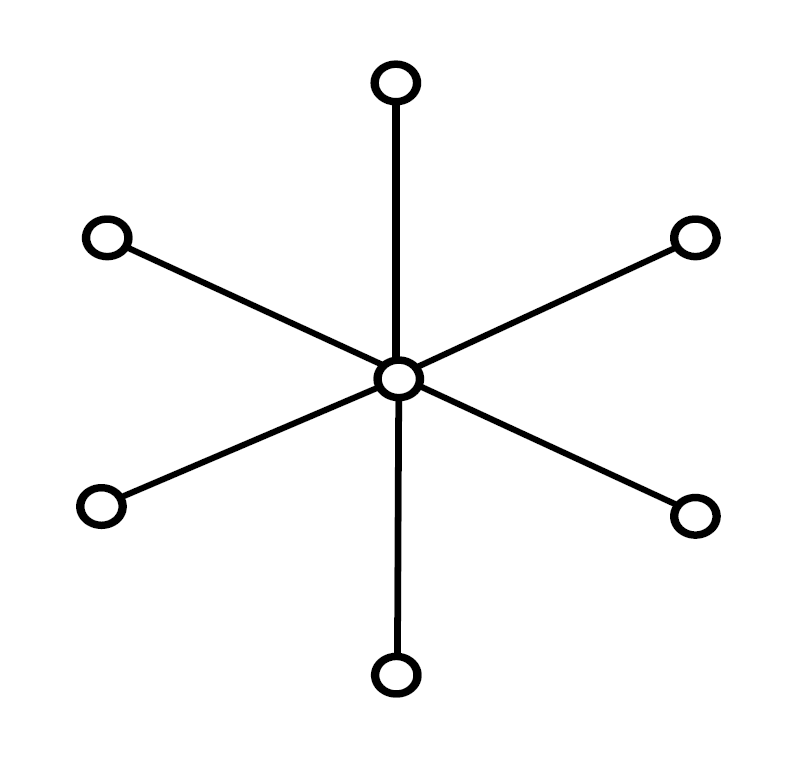
\includegraphics[width=0.2\textwidth]{figs/pblm5.png}
	\caption{Star graph, $K_{1,6}$.}
	\label{fig:pblm5}
\end{figure}

Your task is to show that $K_{1,6}$ can never be an induced subgraph of a $\Delta$-disk proximity graph.










% Problem 6 -------------------------------------------------
% \newpage
\section{}
% \textbf{Problem:}
If $l_{i,j}$ is the shortest path distance (number of edges one needs to follow) between vertices $v_i$ and $v_j$, 
the diameter of the graph is defined as\[
	\diam(G) = \max_{v_i,v_j \in V} l_{i,j}
\] Similarly, if we let $l_{i}^{*}$ (known as the eccentricity of vertex $v_i$) be the longest distance to any vertex from the vertex $v_i$, i.e.,\[
	l_{i}^{*} = \max_{v_j \in V} l_{i,j}
\] then the radius of a graph is defined as\[
	\radius(G) = \min_{v_i \in V} l_{i}^{*}
\] Find the radius and diameter of the following graphs.

\begin{figure}[h]
	\centering
	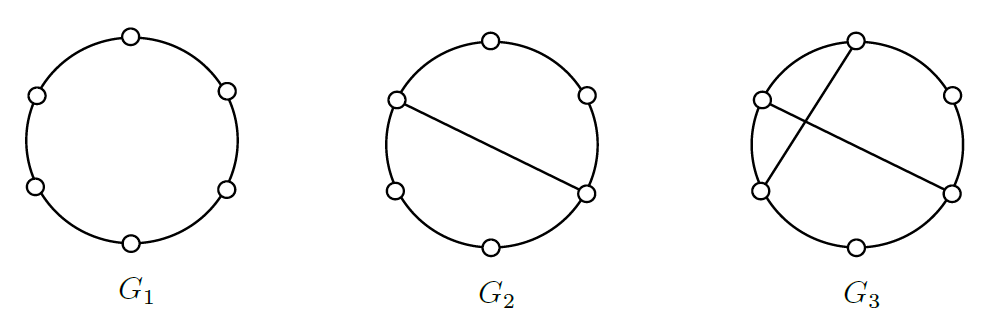
\includegraphics[width=0.7\textwidth]{figs/pblm6.png}
	\caption{Graphs $G_1$, $G_2$, and $G_3$.}
	\label{fig:pblm6}
\end{figure}










% Problem 7 -------------------------------------------------
% \newpage
\section{}
% \textbf{Problem:}
Following are some undirected networks on four nodes with the same initial positions.
In which of these networks, nodes converge fastest under the distributed consensus dynamics? 
Explain your answer.













% Problem 8 -------------------------------------------------
% \newpage
\section{}
% \textbf{Problem:}
What is the necessary and sufficient condition for the consensus to happen in the case of static directed networks? 
Derive this condition.


















% \newpage
% \appendix
% \section{MATLAB Code:}\label{apx:matlab}
% All code I write in this course can be found on my GitHub repository:\\
% \href{https://github.com/jonaswagner2826/MECH6313}{https://github.com/jonaswagner2826/MECH6313}


\end{document}
